\documentclass[10pt]{extarticle}
\usepackage[utf8]{inputenc}
\usepackage{cite}
\usepackage{hyperref}
\usepackage{graphicx}

\title{
    {\large CS2529 Computational Imaging - Project Proposal} \\
    Synthesis of brain tumor MRI images using GAN aggregation with style transfer
}
\author{Sarah Hindawi, Sumant Bagri, Vignesh Edithal}
\date{November 14, 2022}

\begin{document}

\maketitle

\section{Motivation}

\cite{Mukherkjee2022} Proper identification of early stage brain tumors is crucial to prevent long term disability, severe 
cases such as High Grade Glioma may be fatal. Magnetic Resonance Imaging (MRI) is a powerful non invasive tool for obtaining 
these brain scans. MRI scans can provide key information such as the location, shape, size, and growth stage of the brain 
tumor. To perform any medical image analysis using deep learning techniques, a sufficient volume of data with variability is 
required. However, due to constraints such as imaging time and privacy concerns, there is a lack of robust datasets. 
Traditional image augmentation methods (rotation, scale, etc.) create highly correlated images which are unable to capture 
the underlying features of the source images. In addition, they might change the pattern useful for diagnosis. Class 
imbalance is another reason to apply augmentation. Synthetic data generation is a commonly used approach in the field of 
medical image analysis since there is no patient data handling or privacy concerns. Generative Adversarial Networks \textbf
{(GAN)} have shown promising results in generating synthetic data with good generalization and anonymity on a large variety 
of images. We plan to use \textbf{AGGrGAN} \cite{Mukherkjee2022} as it allows us to capture both the unique features of a 
source image using style transfer, and also the shared information among the different latent representations of multiple 
images using aggregation.

\section{Related works}

\cite{Mukherkjee2022} Han et al. \cite{Han2018} have applied DCGAN and WGAN separately on the BraTS 2016 dataset to generate 
artificial MRI scans. To validate their results, they conducted the Visual Turing test with 53\% accuracy for WGAN. Nie et 
al. \cite{Nie2018} have used Fully Convolutional Network (FCN) as generator and a basic CNN as the discriminator, they have 
proposed 3D FCN to estimate target image from the corresponding source image, they have used ADNI dataset and have obtained a 
mean PSNR of 34.1. Emami et al. \cite{Emami2018} have proposed a GAN based model where ResNet is used as the generator and 
discriminator is a CNN with five convolutional layers which classify the image as real or fake, they achieved a mean PSNR of 
26.6 $\pm$ 1.2 for an IRB approved dataset.

\section{Project overview}

Our main goal is to understand how GAN models can help boost research in the medical imaging domain. We aim to implement the
aggregated GAN \textbf{(AGGrGAN)} as described in \cite{Mukherkjee2022} and compare the performance with its component GANs 
(e.g. DCGAN, WGAN) using three metrics, SSIM, PSNR and KL divergence. Subsequently, we will implement style transfer as 
described in \cite{Mukherkjee2022} to improve image resemblance and evaluate its performance both quantitatively (using 
aforementioned metrics) and qualitatively. We plan on introducing the following modifications to AGGrGAN. \textbf{1)} Adding 
a U-Net GAN \cite{Edgar2020}. \textbf{2)} Using two different weight initializations for each GAN (6 GANs in total). \textbf
{3)} Modifying the aggregation algorithm to use images from all GANs instead of picking the top 2 (based on metrics) as 
mentioned in \cite{Mukherkjee2022}. We will perform an ablation study to assess the performance impact of each of these 
modifications. If time permits we would like to implement a basic tumor classification network which will be trained on 
datasets using only real images, only fake images, combination of real and fake images, to show the effectiveness of the 
synthesized images. We will use the publicly available BraTS 2020 \cite{Menze2015} \cite{Bakas2017} \cite{Bakas2018} dataset for our experiments.

\begin{figure} % use [hb] only if necessary!
  \centering
  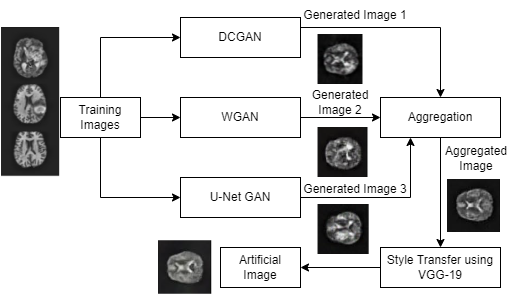
\includegraphics[width=10cm]{AggrGAN_architecture.png}
  \caption{Aggregate GAN (AggrGAN) architecture as implemented in \cite{Mukherkjee2022} with our addition of U-Net GAN}
  \label{AggrGAN_architecture}
\end{figure}

\section{Milestones}

\textbf{Week 1:} Fetch dataset and analyze it for further processing \\
\textbf{Week 2:} Implement DCGAN, WGAN, U-Net GAN and aggregation models \\
\textbf{Week 3:} Implement Style transfer and perform evaluations on the dataset \\
\textbf{Week 4:} Prepare the project report and poster

\bibliographystyle{plain}
\bibliography{proposal}

\end{document}